\section{Optymalizator MySQL}
Praktycznie każde zapytanie SQL skierowane do bazy danych MySQL może zostać zrealizowane na wiele różnych sposobów. Optymalizator jest fragmentem oprogramowania serwera bazodanowego, który odpowiada za wybranie najefektywniejszego sposobu wykonania zapytania (plan wykonania zapytania). W MySQL stosowany jest optymalizator kosztowy, co oznacza, że optymalizator szacuje koszt wykonania dla wariantów planu wykonania i wybiera ten z najmniejszym kosztem. Jednostką kosztu jest odczytanie pojedyńczej, losowo wybranej strony danych o wielkości czterech kilobajtów. Wartość kosztu jest wyliczana na podstawie danych statystycznych, dlatego optymalizator wcale nie musi wybrać najbardziej optymalnego planu. Istnieją dwa rodzaje optymalizacji: \textit{statyczna} i \textit{dynamiczna}. Optymalizacja \textit{statyczna} przeprowadzana jest tylko raz i jest niezależna od wartości. To oznacza, że przeprowadzona raz będzie aktualna nawet jeżeli zapytanie będzie wykonywane z różnymi wartościami. Z drugiej strony optymalizacja dynamiczna bazuje na kontekście, w którym wykonywane jest zapytanie i jest przeprowadzana za każdym razem, kiedy polecenie jest wykonywane. Optymalizacja dynamiczna opiera się na wielu parametrach, takich jak: wartości w klauzuli WHERE czy liczba wierszy w indeksie.

Poniżej przedstawione zostało tylko kilka przykładowych typów optymalizacji, które może wykonać moduł optymalizatora.

\begin{itemize}
	\item \textbf{Zmiana kolejności złączeń}. Podczas wykonywania zapytania tabele nie zawsze są złączane w takiej kolejności jak w zapytaniu. Zagadnienie jest dokładniej opisane w podroździale dotyczącym optymalizatora złączeń.
	\item \textbf{Zamiana OUTER JOIN na INNER JOIN.} OUTER JOIN nie zawsze musi być wykonywany jako OUTER JOIN. Niektóre czynniki takie jak warunki w klauzuli WHERE czy schemat bazy danych mogą spowodować, że OUTER JOIN będzie równoznaczne złączeniu INNER JOIN. 
	\item \textbf{Przekształcenia algebraiczne.} Optymzalizator przeprowadza transformacje algebraiczne takie jak: redukcja stałych, eliminowanie nieosiągalnych warunków czy stałych. Przykładowo warunek (2=2 AND a>2) może zostać przekształcony do postaci (a>2. Podobnie warunek (a<b AND b=c AND a=5) może być przekształcony do (b>5 AND b=c AND a=5).
	\item \textbf{Optymalizacja funkcji MIN(), MAX().}
	Serwer już na etapie optymalizacji zapytania może uznać wartości zwracane przez funkcje jako stałe dla reszty zapytania. W niektórych przypadkach optymalizator może nawet pominąć tabelę w planie wykonania zapytania, jeżeli jedyną wartością pobieraną z tabeli jest wynik funkcji MIN() lub MAX(). W takim przypadku w danych wyjściowych polecenia EXPLAIN znajdzie się ciąg tekstowy "Select tables optimized away".
	Na poniższym przykładzie widzimy, że kolumna \textit{ref} dla pierwszego wiersza jest wartość ''const'', czyli najmniejsza wartość id z tabeli Users została potraktowana jako stała.
	\begin{spverbatim}
		EXPLAIN SELECT * FROM Comments WHERE UserId = (SELECT MIN(id) FROM Users);
	\end{spverbatim}
	\begin{figure}[H]
		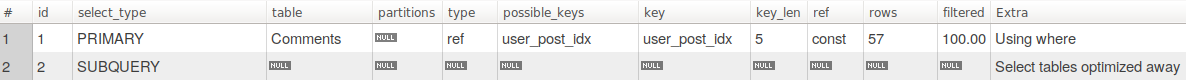
\includegraphics[scale =0.4]{explain20.png} 
	\end{figure}
	\item \textbf{Optymalizacja funkcji COUNT().} Wynik funkcji COUNT(*) bez klauzuli WHERE w niektórych silnikach (np. MyISM), również mogą zostać potraktowane jako stała, ale nie dotyczy to najpopularniejszego obecnie w MySQL silnika InnoDB.
\end{itemize}
////todo opisać więcej przykładów?

\subsection{Dane statystyczne dla optymalizatora}
Przechowywaniem danych statystycznych jest zadaniem silników bazy danych. Z tego powodu w zależności od użytego silnika przechowywane wartości statystyczne mogą być różne. Przykładowo silnik MyISM przechowuje informację o aktualnej liczbie rekordów w tabeli, silnik InnoDB takiej informacji nie przechowuje, natomiast niektóre silniki, np. Archive, w ogólnie nie przechowują danych statystycznych.

 
